% A wrapped history schematic; shades denote age, not spectral magnitude.
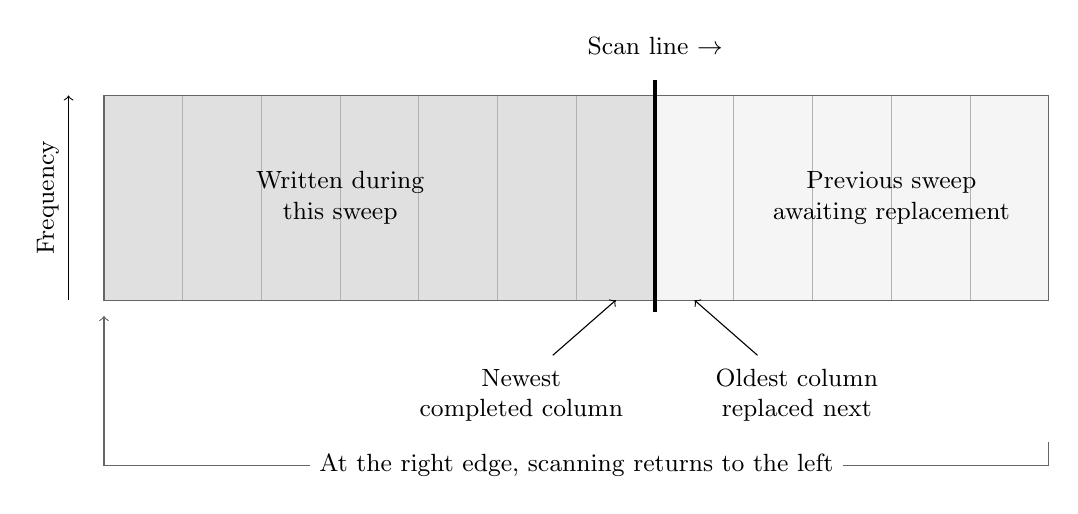
\begin{tikzpicture}[x=1cm,y=1cm,font=\small]
  \fill[black!12] (0,0) rectangle (7,2.6);
  \fill[black!4] (7,0) rectangle (12,2.6);
  \foreach \x in {0,...,11} {
    \draw[black!30] (\x,0) rectangle +(1,2.6);
  }
  \draw[black!60] (0,0) rectangle (12,2.6);
  \draw[very thick] (7,-.15) -- (7,2.8);
  \node[anchor=south] at (7,3) {Scan line $\rightarrow$};
  \node[align=center] at (3,1.3) {Written during\\this sweep};
  \node[align=center] at (10,1.3) {Previous sweep\\awaiting replacement};
  \draw[<-] (6.5,0) -- (5.7,-.7);
  \node[anchor=north,align=center] at (5.3,-.75) {Newest\\completed column};
  \draw[<-] (7.5,0) -- (8.3,-.7);
  \node[anchor=north,align=center] at (8.8,-.75) {Oldest column\\replaced next};
  \draw[->] (-.45,0) -- (-.45,2.6)
    node[midway,above,rotate=90] {Frequency};
  \draw[->,black!60] (12,-1.8) -- (12,-2.1) -- (0,-2.1) -- (0,-.2);
  \node[fill=white] at (6,-2.1) {At the right edge, scanning returns to the left};
\end{tikzpicture}
